\documentclass{article}
\usepackage[margin=1in]{geometry}
\usepackage{mathtools, amsfonts, amsthm, graphicx, listings, xcolor}

\definecolor{codegreen}{rgb}{0,0.6,0}
\definecolor{codegray}{rgb}{0.5,0.5,0.5}
\definecolor{codepurple}{rgb}{0.58,0,0.82}
\definecolor{backcolour}{rgb}{0.95,0.95,0.92}

\lstdefinestyle{mystyle}{
    backgroundcolor=\color{backcolour},   
    commentstyle=\color{codegreen},
    keywordstyle=\color{magenta},
    numberstyle=\tiny\color{codegray},
    stringstyle=\color{codepurple},
    basicstyle=\ttfamily\footnotesize,
    breakatwhitespace=false,         
    breaklines=true,                 
    captionpos=b,                    
    keepspaces=true,                 
    numbers=left,                    
    numbersep=5pt,                  
    showspaces=false,                
    showstringspaces=false,
    showtabs=false,                  
    tabsize=2
}

\lstset{style=mystyle}

\title{Title}
\author{Sam Ly}


\begin{document}
\maketitle

\section*{Q1 (5 pts)}

\begin{enumerate}
    \item {
        Draw the graph.
        \begin{figure}[htbp]
            \centering
            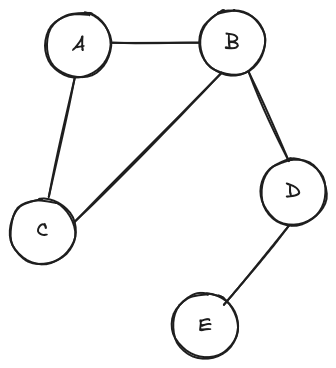
\includegraphics[width=0.4\textwidth]{graph.png}
        \end{figure}
    }

    \item {
        Compute the degree of each node.

        \[ \text{deg}(A) = 2 \]
        \[ \text{deg}(B) = 3 \]
        \[ \text{deg}(C) = 2 \]
        \[ \text{deg}(D) = 2 \]
        \[ \text{deg}(E) = 1 \]
    }

    \item {
        Verify the \textbf{Handshake Theorem}.

        \[\sum_{v \in V}{\text{deg}(v)} = 2 |E| \]

        \[2+3+2+2+1 = 10 = 2 |E| \]
    }

    \item {
        Explain briefly why this must always hold for undirected graphs.

        This must always hold true for undirected graphs because each edge
        always connects two nodes. This means those two nodes increase their
        degree by one when connected by one edge. By extension, each edge 
        increases the sum of all node degrees. 

        Therefore, the sum of all degrees of nodes is equal to two times the 
        number of edges.
    }
\end{enumerate}

\section*{Q2 (5 pts)}

\begin{enumerate}
    \item {
        Write down the \textbf{degree distribution}: how many nodes have degree 1, 2, 3, etc.

        \begin{table}[htbp]
            \centering
            \begin{tabular}{ll}
                Degree & No. of Nodes \\
                1 & 1 \\
                2 & 3 \\
                3 & 1 \\

            \end{tabular}
        \end{table}
    }

    \item {
        Write a short \textbf{Python snippet} that:
        \begin{itemize}
            \item Stores the graph as a dictionary of neighbors.
            \item Loops over nodes to compute degrees.
            \item Prints the degree distribution.
        \end{itemize}

        \lstinputlisting[language=Python]{./code/script.py}        
    }
\end{enumerate}

\end{document}